\documentclass[main.tex]{subfiles}

\begin{document}
    
\section{Iterative solvers in 2D}

This section goes through necessary parts needed to build a V-cycle solver on a 2D grid with the same assumptions as in section 2. Without further ado, let's take a look at a pseudoalgorithm first and then explain what individual functions do in detail.
\begin{algorithm}[h]
    \underline{function Vcycle($U, \omega, n_{smooth}, m, F$)}\\
    \eIf{$m = 1$}
    {
        directly solve at the coarsest level
    }
    {
        pre-smoothing: \texttt{smooth}\\
        compute the residual: $r = F - A u$\\
        coarsen residuals: \texttt{coarsen}\\
        recursive part to obtain error: \texttt{Vcycle($\mathbf{0}, \omega, n_{smooth}, -R_{coarse}$)}\\
        interpolate the error: \texttt{interpolate}\\
        update the solution: $U = U + E$\\
        post-smoothing: \texttt{smooth}\\
    }
    \textbf{return} U
    \caption{V-cycle algorithm pseudocode, full reference can be found on slide 8 of Lecture 20 or in LeVeque 4.6.2 ``The multigrid approach''}
\end{algorithm}
The name V-cycle comes from the recursive part of the algorithm -- the 2 lines indicate the path of pre- and post-smoothing on coarse/interpolated grids, whereas the point of the intersection indicates directly finding the solution in the first \texttt{if} branch.

It is worth noting that due to coarsened grid the depth of the recursion will be $\log_2(m)$ per one cycle. The cycle will be repeated until a desired tolerance is reach or the maximum number of iterations has passed.

\subsection{Matrix free 5-point Laplacian}
As requested in the handout, matrix-free method \texttt{Amult} will be used to calculate the term $\mathbf{-A u}$ without storing the $\mathbf{A}$ matrix in memory (as it is of size $m^2 \times m^2$ and somewhat sparse). The implementation can be tested with Matlab's Conjugate Gradient algorithm \texttt{pcg}, which can accept a function handle as the first argument, so \texttt{Amult} shall be provided. The reason why $-\mathbf{A u}$ is used instead of the positive alternative is that PCG requires a positive definite system and the $\mathbf{A}$ matrix is in fact negative definite.
\begin{figure}[h]
    \centering
    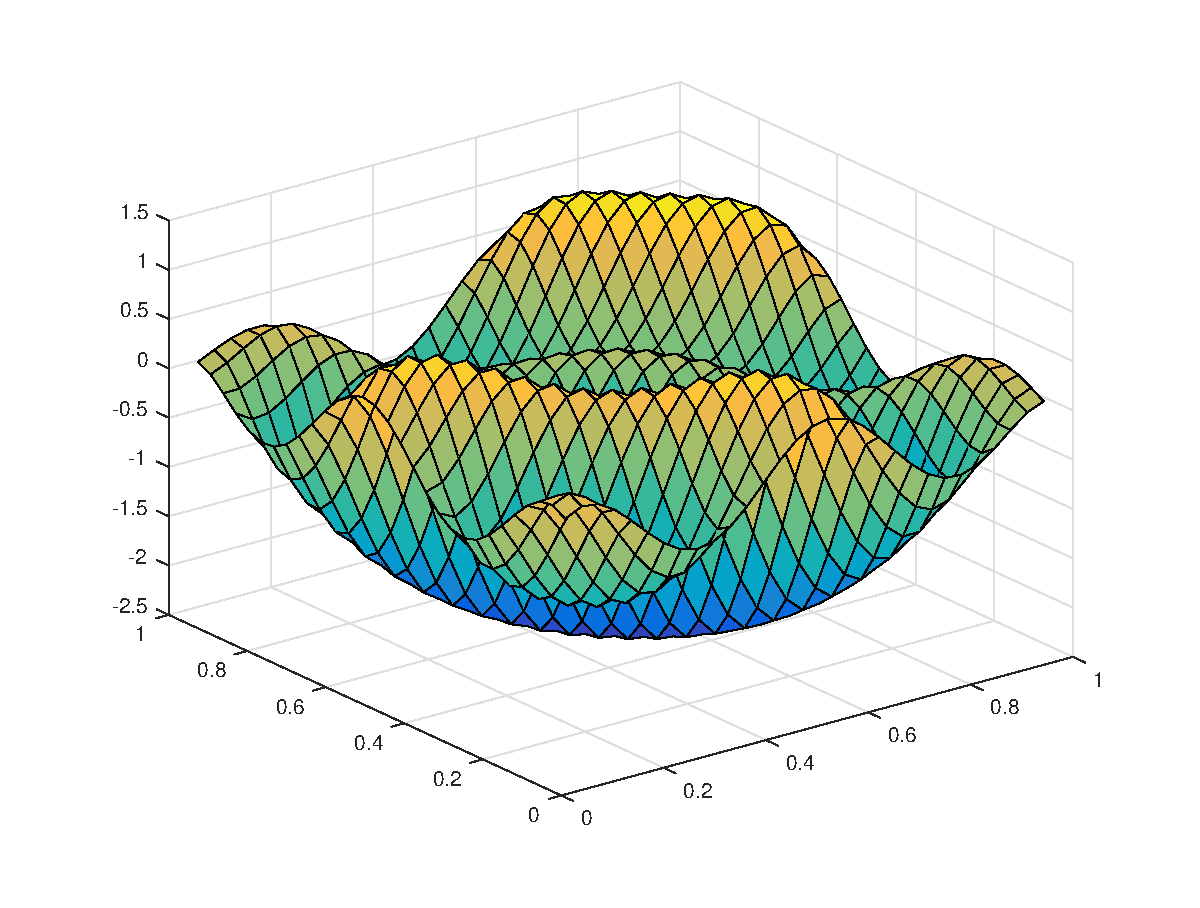
\includegraphics[width=\textwidth]{../Figures/ex31}
    \caption{Solution to $-\mathbf{A u} = -\mathbf{f}$ using PCG}
\end{figure}
To check the difference between the implementation of the matrix free method and the direct multiplication of $u$ with the Laplacian matrix, one can for example use \texttt{max(max(abs(Amult(u,m) - -1*poisson5(m)*u)))} in Matlab. The maximum of the absolute difference is roughly $10^{-12}$.

All the Matlab code for this section is provided in the appendix. 

\subsection{Relaxation and smoothing}
The main motivation to use underelaxed Jacobi is that while the high frequency components of the error decay after a few iterations when applying the ordinary Jacobi method, the lower frequency components remain longer and negatively affect the convergence of the algorithm.

Thereby, by including an extra parameter $\omega$ we can manage how far the current iterate moves towards the true solution, and thus control high frequency harmonics.

\begin{equation}
G_\omega = (1-\omega)I + \omega G
\end{equation} 

where $G$

\begin{equation}
G = I + \frac{h^2}{2} A
\end{equation}

besides, considering that the eigenvectors of $G$ are the same as the eigenvectors of $A$

\begin{equation}
\rho_{p,q} = 2 + \frac{h^2}{2} \lambda_{p,q}
\end{equation}

from 3.15 in Leveque we know that the eigenvalues of $A$ are

\begin{equation}
\lambda_{p,q} = \frac{2}{h^2}((cos(p \pi h) -1) + (cos(q \pi h) -1 ))
\end{equation}

thus, combining the equations above we obtain the following expression for the eigenvalues of $G_\omega$

\begin{equation}
\gamma_{p,q} = (1-\omega) + \omega ( cos(p \pi h) + cos(q \pi h))
\end{equation}

and since we would like to choose $\omega$ so that we get optimal smoothing of high frequencies

\begin{equation}
\omega_{opt} = min ( max |\gamma_{p,q}|)
\end{equation}

Figure \ref{fig:omegaopt} shows $max |\gamma_{p,q}|$ for different values of the smoothing factor. We see in this case that $\omega_{opt}$ lies very close to $0.5$.

\begin{figure}[h]
    \centering
    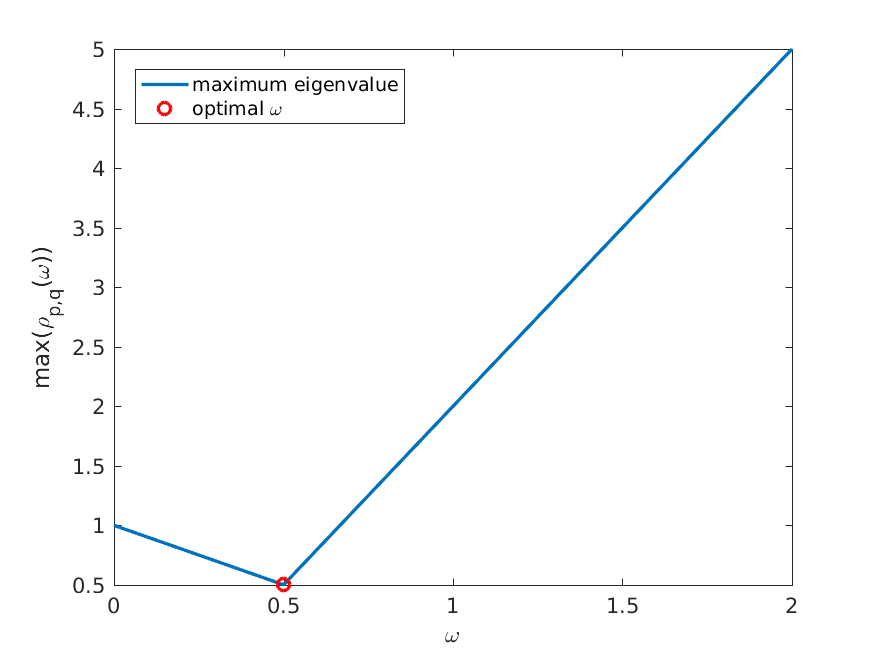
\includegraphics[width=\textwidth]{../Figures/omegaopt}
    \caption{$max |\gamma_{p,q}|$ for different values of $\omega$ and $m = 1000$}
    \label{fig:omegaopt}
\end{figure}

We have implemented a script in MATLAB that plots $max |\gamma_{p,q}|$ as a function of $\omega$ and finds the minimum of that function. We also wrote the function smooth which applies the under/overrelaxed Jacobi method for a given value of the smoothing parameter.

\subsection{Coarsing / interpolating}
To further continue, a necessary part of the V-cycle is coarsing and interpolation of the grid. As is mentioned in the book, the convergence rate for some components of the error is greatly improved by transferring the error to a coarser grid. An example is given that a component's frequencies can be shifted to the right, i.e. more in the middle of what range the coarse grid has to offer, resulting in the improvement of the damping factor (in some cases as high as one order of the magnitude).

There are multiple approaches to coarsion and interpolation on an evently spaced squared grid. The simplest one is taking every second point of the original grid in coarsion and calculating back the points of interpolated grid as a weighted average of the neighbouring points. In this approach three possible scenarios can happen to calculate the interpolated point: adding 2 neighbours vertically, adding 2 neighbours horizontaly and finally, adding 4 neighbours located in NE, NW, SE, SW.

\subsection{Recursion}
Now the problem is refolmulated in order to transfer the remaining part to the coarser grid. The approach taken uses the recursive call to find the error vector by solving $\mathbf{A e} = \mathbf{-r}$ via the \texttt{vcycle} method.

Since the result is obtained on a coarse grid, interpolating is used in order to project the error vector back to the original grid. In order to find a better approximation of $U$ the error vector is added and post-smoothing is performed. Once all the recursive results are popped from the stack a solution to the given problem is returned. As mentioned before this process is repeated until a desired tolerance or maximum number of iterations is reached. 

\subsection*{Conclusion}
With the initial parameters for the V-cycle driver and number of smoothing iterations set to 1000, 23 iterations are needed to reach the desired tolerance of $1^{-10}$. Increasing the aforementioned number of smoothing interations results in longer computational time, but decreases the overall number of steps needed for convergence. As can one expect lowering $k$ in $m=2^k - 1$ yields considerably less iterations, for example for $k=5$, only 5 run throughs of the for-loop are executed. Having a larger grid would naturally increase the computation time.

\begin{figure}[h]
    \centering
    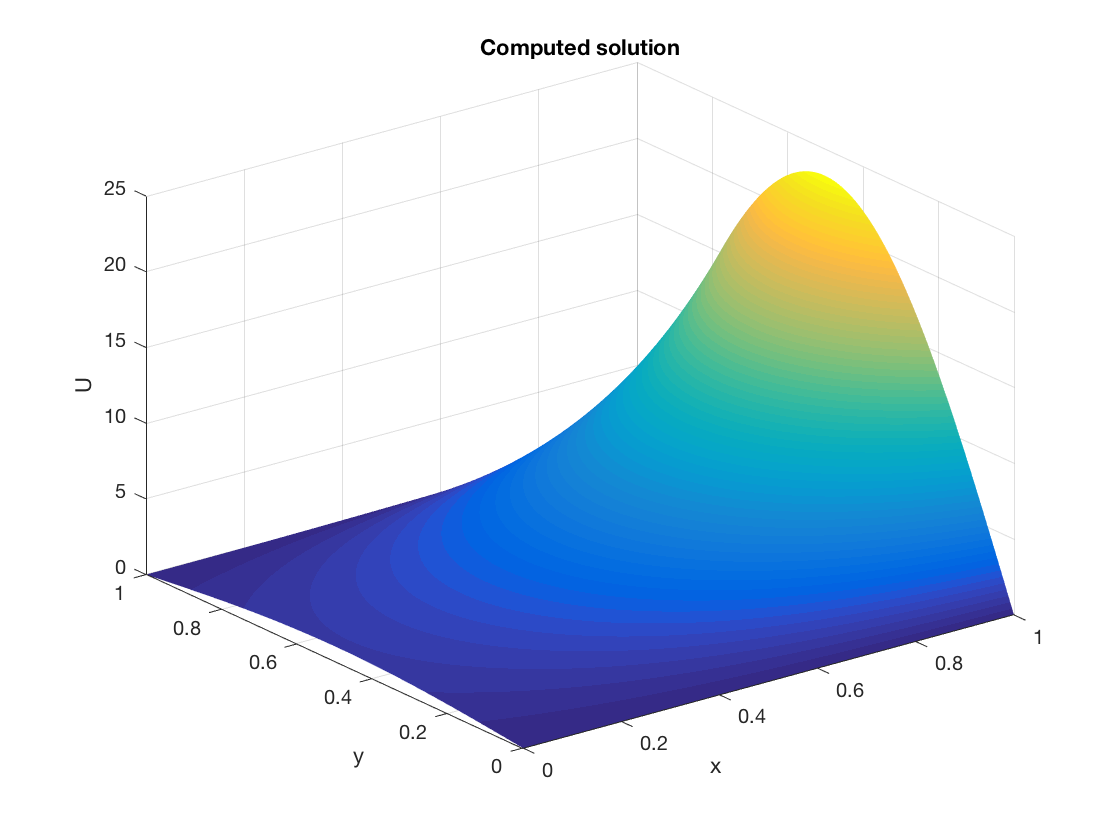
\includegraphics[width=\textwidth]{../Figures/ex33.png}
    \caption{Result of 23 Vcycles with the default parameters}
\end{figure}

Further work can be done to implement the W-cycle or other ways of coarsion and interpolation, such as using a stencil like shape to weigh the grid points.
    
\end{document}